\documentclass[a4paper,11pt]{refart}
\usepackage{listingsutf8}
\usepackage[brazilian]{babel}%Sinais e pountuação em portugês
\usepackage[utf8]{inputenc}
\usepackage[T1]{fontenc} % LY1 also works
\usepackage{tikz}
\usetikzlibrary{shapes,arrows}
%% Font settings suggested by fbb documentatio
\usepackage{float} 
\usepackage{listings}
\usepackage{microtype}
\usepackage{graphicx}
\usepackage{enumitem}
\setlist{leftmargin=*}
\lstset{basicstyle=\ttfamily,frame=single,xleftmargin=1em,xrightmargin=1em}
\usepackage[os=win]{menukeys}
\renewmenumacro{\keys}[+]{shadowedroundedkeys}
\usepackage{framed}
\usepackage{etoolbox}
\AtBeginEnvironment{leftbar}{\sffamily\small}
\usepackage[T1]{fontenc}
\usepackage{lmodern}
\usepackage{hyperref}
\usepackage{multirow}                                               
\usepackage{multicol}                                               
\usepackage{longtable}
\usepackage{amsmath}
\usepackage{dcolumn}
\usepackage{booktabs}
\usepackage{makecell}
\hyphenation{Trans-fe-rên-cias} %Hifenação de palavras

\hypersetup{colorlinks=true,linkcolor=black,citecolor=blue,urlcolor=blue}

\renewcommand\theadalign{bc}
\renewcommand\theadfont{\bfseries}
\renewcommand\theadgape{\Gape[4pt]}
\renewcommand\cellgape{\Gape[4pt]}


\def\CS#1{\texttt{\textbackslash#1}}

\usepackage[most]{tcolorbox}
\newtcblisting{commandshell}{colback=black,colupper=green,colframe=black!75!black,
	listing only,listing options={style=tcblatex,language=sh},
	every listing line={\textcolor{red}{\small\ttfamily\bfseries computer@user:\$ }}}

\usepackage[most]{tcolorbox}
\newtcblisting{shell}{colback=black,colupper=green,colframe=black!75!black,
	listing only,listing options={style=tcblatex,language=sh},
	every listing line={\textcolor{red}{\small\ttfamily\bfseries  }}}

\usepackage[most]{tcolorbox}
\newtcblisting{pymol}{colback=white,colupper=black,colframe=gray!75!black,
	listing only,listing options={style=tcblatex,language=sh},
	every listing line={\textcolor{red}{\small\ttfamily\bfseries  }}}



\title{ \huge {PRIMoRDiA Tutoriais: XI EMMSB} }
\author{Igor Barden Grillo \\(\url{barden.igor@gmail.com} )\\\url{github.com/bardenChem}}

\begin{document}
	\maketitle
	
	
	\hspace*{-1.2\leftmarginwidth}
	\begin{minipage}{\fullwidth}
		\begin{figure}[H]
			\begin{center}
				\includegraphics[width=7in]{logo_primordia}
			\end{center}
		\end{figure}	
	\end{minipage}	
	\newpage
	
	\newpage
	\tableofcontents
	\newpage
	
	\section*{Introdução}
	
	
	Esse documento contém os tutoriais para o programa PRIMoRDiA direcionados para a XI edição da Escola de Modelagem Molecular de Sistemas Biológicos (EMMSB) do Laboratório Nacional de Computação Científica (LNCC). 
	
	O PRIMoRDiA ( \textbf{PRI}MoRDiA \textbf{M}acromolecular \textbf{R}eactivity \textbf{D}escriptors \textbf{A}ccess ) é um software escrito em \emph{C++}, desenvolvido para o pós-processamento eficiente dos resultados de pacotes de química computacional, produzindo uma grande variedade de descritores quânticos: propriedades eletrônicas e reatividade de sistemas químicos. 
	
	O PRIMoRDiA traz implementado os principais descritores de reatividade da Teoria do DFT conceitual, incluindo as definições matemáticas para as teorias de elétrons de fronteira de Fukui e de ácidos e bases duros e moles de Pearson. O PRIMoRDiA foi desenvolvido com foco no cálculo de descritores e outras propriedades eletrônicas mais comuns para grandes moléculas que são relevantes para processos biológicos, e por isso há descritores modificados especificativamente para atender as particularidades desses sistemas. 
	
	Também oferecemos um guia de usuário com informações gerais sobre a teoria e detalhes sobre o uso e interpretação dos resultados gerados pelo programa.  PRIMoRDiA foi desenvolvido na Universidade Federal da Paraíba, no Laboratório de Química Quântica e Computacional. Nosso grupo possui uma série de trabalhos já publicados, como a referência principal do programa , aplicações para a caracterização teórica de reações de catálise enzimática \cite{grillo_primordia_2020}, uma revisão sobre a exploração da estrutura eletrônica de macromoléculas biológicas usando métodos semi-empírico para os cálculos quânticos\cite{grillo_quantum_2023}, aplicações para ligante e proteína\cite{grillo_semiempirical_2020,rocha-santos_thermochemical_2021}, e outras aplicações\cite{grillo_elucidating_2020,grillo_theoretical_2020}.
	
	Os tutoriais nesse documento cobrem as funcionalidades relacionadas com o estudo da estrutura eletrônica de macromoléculas, mais especificamente proteínas, e a análise teórica de reatividade de reações enzimáticas, assim como também a obtenção de um caminho de reação enzimático para realizar o mesmo. 
	
	Utilizar o PRIMoRDiA é muito simples, consiste geralmente em duas etapas, sendo a primeira a montagem do arquivo de input, no qual o programa também ajuda a fazer, e a segunda a parte de execução dos cálculos. Por isso, os tutorias aqui apresentados tem com objetivo maior de apresentar os resultados do PRIMoRDiA e como utilizar esses dados para aplicar em problemas de pesquisa.
		
	\section{Tutorial 1: Descritores de Banda - Aplicação para Ligante Proteína}
	
	No documento de tutoriais do PRIMoRDiA encontramos no tutorial de número 3 como executar os cálculos e as análises de descritores quânticos de reatividade para sistemas macromoleculares de relevância biológica, que obrigatoriamente precisam ter sua estrutura tridimensional codificada em um arquivo de PDB. No exemplo do tutorial original, os cálculos exploram todas as opções possíveis para sistemas de teste, polipeptídeos de aproximadamente 300 átomos,  que não possuem im interesse de pesquisa significativo. No presente tutorial, serão aplicados os cálculos em complexos entre a enzima RTA (Ricin Toxic A chain) e ligantes que tem potencial inibidor já descritos experimentalmente. Mais precisamente, nesse tutorial vamos recriar resultados teóricos de um dos artigos de pesquisa do nosso grupo\cite{rocha-santos_thermochemical_2021}. 
	
	\subsection{Arquivos Necessários e Execução do Programa}
	
	Nesse tutorial aproveitaremos os resultados de cálculos semi-empíricos dos tutoriais anteriores desse minicurso, onde vamos fazer os cálculos do PRIMoRDIA para os complexos de RTA com o ligante 19M e JP3. Para cada um desses arquivos tem um arquivo de PDB, que contém as informações relevantes ao biopolímero que vai ser utilizado pelo PRIMoRDiA para escrever descritores e representações especiais.
	
	Para facilitar a produção de input a partir desses arquivos vamos usar o seguinte comando, na pasta onde contém os arquivos ".aux" dos complexos que serão analisados
	
	\hspace*{-1.2\leftmarginwidth}
	\begin{minipage}{\fullwidth}
		\begin{commandshell}path/to/PRIMoRDiA_1.25v -input -op 3 -p mopac\end{commandshell}
	\end{minipage}
	
	
	Um arquivo de chamado de primordia.input é gerado na pasta. A primeira \textit{keyword} encontrada no arquivo é "\#RT normal" para indicar que o Run Type (tipo de cálculo) é do tipo comum esperado para a execução do PRIMoRDiA. O keyword "\#PR" indica os que as próximas entradas na linha são parâmetros especiais, que no caso, por hora, é "eband" e "1", indicando que o limite para considerar orbitais moleculares em relação HOMO-LUMO é de 1eV. As duas linhas que começam com o inteiro "3", indicam a opção de cálculo do PRIMoRDiA especial para macromoléculas. Vamos editar  o aqruivo em um editor de texto para conter as informações como mostrado na caixa de texto abaixo
	
	\hspace*{-1.5\leftmarginwidth}
	\begin{minipage}{\fullwidth}
		\begin{lstlisting}[caption={Input editado para execução do tutorial 3},label={tut301}]
#RT normal 
#PR eband 1 extrard pymols 
3 jp3_complex.aux true 0 0 jp3.pdb mopac 0 0 0 0  EW 
3 19m_complex.aux true 0 0 19m_complex.pdb mopac 0 0 0 0 EW	
		\end{lstlisting}
	\end{minipage}
	
	Esses argumentos são detalhadamente explicados no guia do usuário, mas também são descritos um por um na lista abaixo
	
	\begin{itemize}
		\item "3" : Indica a opção de cálculo dos descritores para o PRIMoRDiA
		\item "jp3\_complex.aux": Nome do arquivo de output que contém a informação de estrutura eletrônica
		\item "true" : Keyword para opção de dureza local para ser calculada na versão volumétrica
		\item "0" : Granularidade/resolulção dos arquivos de cube a serem gerados para os descritores volumétricos, zero indica que esses cálculos de grid não serão gerados.
		\item "0" : Número máximo de orbitais moleculares a ser utilizados pelo método BD
		\item "jp3\_coplex.pdb": Nome do PDB com as informações de referência
		\item "0" : Coordenada do eixo x para o centro da caixa a ser gerado para os descritores volumétricos
		\item "0" : Coordenada do eixo y para o centro da caixa a ser gerado para os descritores volumétricos
		\item "0" : Coordenada do eixo z para o centro da caixa a ser gerado para os descritores volumétricos
		\item "0" : Tamanho do lado da caixa a ser gerada a partir do centro dado pelas coordenadas acima
		\item "EW" : Keyword para sinalizar o método de cálculo de descritores para macromoléculas ponderado por energia
	\end{itemize}
	
	Para a produção de arquivos cube, com dados volumétricos, é possível limitar uma área de cálculo para obter uma definição maior com menor custo computacional. Para isso é necessário definir um caixa onde o grid vai ser calculado, o centro e o tamanho dados no arquivo de input, como foi indicado acima. Nos dados originais da publicação não utilizamos os arquivos cube, por ser mais útil mapear esses descritores por átomo devido a quantidade de elementos para serem representados nas imagens.  
	
	O PRIMoRDiA tem implementado dois métodos para combinar esse orbitais moleculares:
	
	\begin{enumerate}
		\item Band Density (BD: sigla e Keyword utilizada dentro do programa)
		\item Energy weighted (EW: sigla e Keyword utilizada dentro do programa)
	\end{enumerate}
	
	O primeiro é inspirado no cálculo de densidade eletrônica, com a particularidade de considerar somente uma seleção de orbitais moleculares a partir do HOMO, para os ocupados, e LUMO para os virtuais. O segundo é uma combinação que é ponderada pela diferença de energia dos orbitais moleculares dos orbitais de fronteira HOMO-LUMO. Há um limite para considerar esses orbitais que é definido por um valor de corte de energia definido pelo usuário.
	
	Nesse exemplo, vamos rodar os dois sistemas com o método \textit{EW}, que foi utilizado na publicação do nosso grupo, mas como desafio, esses cálculos podem ser feitos com o método \textit{BD}.	Finalmente, com esse input podemos colocar o programa para rodar com o seguinte comando
	
	
	\hspace*{-\leftmarginwidth}
	\begin{minipage}{\fullwidth}
		\begin{commandshell}path/to/PRIMoRDiA_1.25v -f primordia\_editado.input\end{commandshell}
	\end{minipage}
	
	Usamos o arquivo "primordia\_editado.input", que foi editado a partir do arquivo automático gerado pelo software.
	O programa deve finalizar a sua execução sem erros e produzir vários arquivos no diretório, com extensão ".cube', ".pym", ".lrd" e etc. Vamos explicar os arquivos com os resultados de descritores e como analisá-los na próxima seção desse tutorial.
	
	\subsection{Análise dos Resultados}	
	
	Dos resultados produzidos temos os descritores globais, locais em representação condensada (arquivos ".lrd"), locais em representação volumétrica (arquivos ".cube", não gerados nesse tutorial) e locais condensados escritos em PDB (nas pastas "RD\_PDB"). Para macromoléculas é interessante observar os descritores globais por uma questão de acompanhamento da normalidade do cálculo quântico executado, pois os processos nesses sistemas tendem a ser somente locais, tendo pouca relevância a propensão de uma proteína inteira de transferir ou receber elétrons. Por isso não vamos analisar do arquivo "primordia.global".
	
	Para esse lançamento estável do programa, PRIMoRDiA 1.25v, a principal modificação é a consolidação dos scripts de automatização de análise e produção de resultados com qualidade de publicação, usando o pacote gráfico Pymol e o pacote estatístico R. Por isso, nos próximos passos do tutorial, vamos focar na produção de imagens a partir desses scripts.
	
	No entanto, esse tipo de representação pode ser bem complicada de trabalhar, já que é uma lista de valores por átomos, ou seja, uma tabela que pode ser significativamente grande para macromoléculas. Pensando em facilitar a análise dessas resultados, o PRIMoRDiA escreve um arquivo de PDB para cada descritor calculado com os valores no campo do b-factor, e assim podemos usar o pacote gráfico Pymol para visualizar os descritores colorindo os átomos com uma paleta customizada. Para operar o Pymol mais automaticamente possível, o PRIMoRDiA escreve um arquivo de script com o sufixo "\_pymols\_pdb.pym", com um exemplo de sua estrutura mostrado na \autoref{rta_pymols}.
	
	\hspace*{-\leftmarginwidth}
	\begin{minipage}{\fullwidth}
		\begin{figure}[H]
			\begin{center}
				\includegraphics[width=4in]{rta_pymols}
				\caption{Script de automação da visualização dos descritores locais condensados no Pymol escrita no PRIMoRDiA e aberta em editor de texto.}
				\label{rta_pymols}
			\end{center}
		\end{figure}
	\end{minipage}

	Esse arquivo tem comandos para executar no Pymol modificando parâmetros de visualização e para carregar os PDBs com os descritores. Além disso ele já executa algumas paletas de cores, sendo que uma vai sobrepondo a outra, mas servem para o usuário pegar e escolher uma ou modificar seus parâmetros e cores. Vamos começar abrindo o seu Pymol, execute o comando mostrado a baixo

	\hspace*{-\leftmarginwidth}
	\begin{minipage}{\fullwidth}
		\begin{pymol}@19m_pymols_pdb.pym\end{pymol}
	\end{minipage}

	Depois da execução desse comando, a janela do pymol deve abrir e carregar todos os arquivos de PDB e executar todos os comandos que configuram a paleta de cores baseada nos valores dos descritores (\autoref{pymol_window}) . O último comando de "spectrum b..." executada deve ser o que fica aparecendo, como na \autoref{pymol_window2}.

	\hspace*{-\leftmarginwidth}
	\begin{minipage}{\fullwidth}
		\begin{figure}[H]
			\begin{center}
				\includegraphics[width=5in]{pymol_window}
				\caption{Janela do Pymol com o comando para executar}
				\label{pymol_window}
			\end{center}
		\end{figure}
	\end{minipage}


	\hspace*{-\leftmarginwidth}
	\begin{minipage}{\fullwidth}
		\begin{figure}[H]
			\begin{center}
				\includegraphics[width=5in]{pymol_window2}
				\caption{Descritores locais condensados para a estrutura do complexo 19M 	carregados no Pymol.}
				\label{pymol_window2}
			\end{center}
		\end{figure}
	\end{minipage}

	Na próxima imagem nós mostramos o Pymol com somente um dos objetos ativos, o 19M\_complex\_netphilicity, e mostrando o comando a ser executado no terminal, que foi selecionado/copiado a partir de um daqueles que foi executado quando o script foi chamado.


	\hspace*{-\leftmarginwidth}
	\begin{minipage}{\fullwidth}
		\begin{figure}[H]
			\begin{center}
				\includegraphics[width=5in]{pymol_window3}
				\caption{Janela do Pymol mostrando o objeto 19M\_complex\_netphilicity ativo e o comando para gerar a paleta de cores.}
				\label{fig_tut3_6}
			\end{center}
		\end{figure}
	\end{minipage}

	Esse descritor mostra as regiões propensas a receber um ataque nucleofílico nos valores positivos, pintados em tons de vermelho, portanto demonstra o potencial local de eletrofilicidade desses átomos. Nos valores negativos, pintados em tons de azul, não aparecem nessa imagem pois os átomos propensos a ataques eletrofílicos, portanto, com um potencial local de nucleofilicidade, não estão destacados nessa imagem. Mas, para chegar em uma imagem semelhante a que foi para o artigo publicado, vamos analisar para esse complexo o descritor de dureza local, mais precisamente com a aproximação de Fukui-à-esquerda, que é a função que representa a porção da densidade eletrônica mais propensa a ser transferida e que substitui a densidade eletrônica total no cálculo de dureza. 
	
	Na \autoref{19_hardness_w}, é mostrado a janela com o objeto com o descritor de dureza mencionado já selecionado e com a paleta de cores que é geralmente escolhida pelo nosso grupo. Vamos explorar o comando mostrado na tela para gerar uma imagem com uma visualização ainda mais aprimorada que a figura que foi publicado no estudo de 2021.
	
	\hspace*{-\leftmarginwidth}
	\begin{minipage}{\fullwidth}
		\begin{figure}[H]
			\begin{center}
				\includegraphics[width=5in]{19m_hardness_window}
				\caption{Janela do Pymol mostrando o objeto de potencial de Fukui Left ativo e o comando para edição da paleta de cores mostrada no campo de comando.}
				\label{19_hardness_w}
			\end{center}
		\end{figure}
	\end{minipage}

	Vamos selecionar o ligante e ativar a visualização das esferas\autoref{19_hardness_spheres} e ajustar as cores, usando como mínimo o valor de 0.15 e máximo de 0.23. Isso vai fazer com que se destaque mais a diferença entre os átomos e distinguir os mais propensos a interações duro-duro. Também, para aprimorar a renderização da imagem final, vamos mudar o modo de tracejado com o seguinte comando 
	
	\hspace*{-\leftmarginwidth}
	\begin{minipage}{\fullwidth}
		\begin{pymol}set ray_trace_mode=1\end{pymol}
	\end{minipage}
	
	\hspace*{-\leftmarginwidth}
	\begin{minipage}{\fullwidth}
		\begin{figure}[H]
			\begin{center}
				\includegraphics[width=5in]{19_complex_show_spheres}
				\caption{Janela do Pymol mostrando o ligante selecionado e o menu com opção para mostrar a representação de esferas para os átomos.}
				\label{19_hardness_spheres}
			\end{center}
		\end{figure}
	\end{minipage}
	
	
	 E depois, para renderizar a imagem em máxima qualidade, usamos o comando "ray", como mostrado abaixo
	 
	 \hspace*{-\leftmarginwidth}
	 \begin{minipage}{\fullwidth}
	 	\begin{pymol}ray antialias=2\end{pymol}
	 \end{minipage}
	 
	 Depois do comando "ray", é possível estabelecer os valores em pixels da imagem e controlar isso também. A opção "antialias=2" estabelece a maior qualidade para a renderização de imagens. Depois de renderizar a imagem, a janela do Pymol fica como na \autoref{19_ray}, e pode ser salva com o comando abaixo
	
	\hspace*{-\leftmarginwidth}
	\begin{minipage}{\fullwidth}
		\begin{pymol}png complex_rta_19m_hardness.png\end{pymol}
	\end{minipage}
	

	\hspace*{-\leftmarginwidth}
	\begin{minipage}{\fullwidth}
		\begin{figure}[H]
			\begin{center}
				\includegraphics[width=5in]{19m_ray}
				\caption{Janela do Pymol com a estrutura renderizada e pronta para ser salva.}
				\label{19m_ray.}
			\end{center}
		\end{figure}
	\end{minipage}

	O resultado é mostrado na \autoref{19m_hardness_improoved}, em uma imagem que consegue mostras bem os átomos mais duros, baseado no potencial de Fukui, diferenciando bem os grupos farmacofóricos do ligante 19M.  
	
	\hspace*{-\leftmarginwidth}
	\begin{minipage}{\fullwidth}
		\begin{figure}[H]
			\begin{center}
				\includegraphics[width=5in]{19m_hardness_improoved}
				\caption{Imagem final renderizada do potencial de Fukui-Esquerdo para o complexo RTA-19M.}
				\label{19m_hardness_improoved}
			\end{center}
		\end{figure}
	\end{minipage}


	\newpage
	\section{Tutorial 2: Gerando Trajetória de Catálise Enzimática}
	
	Um dos usos mais recorrentes do PRIMoRDiA, e portanto, da análise de estrutura eletrônica para macromoléculas, é a caracterização teórica de caminhos de reação enzimático. O que isso significa na prática é basicamente uma análise de reatividade e interações químicas contidas no sítio ativo de uma enzima com o substrato que se queira analisar, para cada etapa da reação catalisada. Isso permite obter uma visão teórica geral sobre os fenômenos químicos que ocorrem antes, durante e após esses processos tão essenciais para a manutenção dos organismos vivos, identificar os papéis de resíduos, íons, e corroborar informações de obtidas as simulações de caminhos de reação, como ordem das coordenadas de reação e  sentido das transferências eletrônicas.
	 
	Apesar de tudo isso que pode ser obtido com os cálculos efetuados pelo PRIMoRDiA, é necessária a determinação prévia de uma trajetória de estruturas, que representem um caminho de reação química. Por isso, esse tutorial tem como objetivo mostrar a utilização de scripts em Python 3 desenvolvidas pelo nosso grupo para operar facilmente a biblioteca pDyanmo, que permite realizar cálculos de de potencial Híbrido de Mecânica Quântica/Mecânica Molecular, que é o tipo de protocolo mais comum para simulação de reações químicas em grandes sistemas biológicos. 
	
	\subsection{O Sistema: Triose-Fosfato Isomerase} 
	
	Reações enzimáticas são reações químicas catalisadas por proteínas, que fazem com que transformações químicas ocorram em um tempo hábil para o funcionamento do metabolismo de organismos vivos. Portanto, as enzimas são componentes importantíssimos para a manutenção da vida, participando desde a replicação de DNA até a decomposição do açúcar.
	
	O estudo do mecanismo dessas reações é muito importante para o desenvolvimento de drogas, entendimento de metabolismo, mecanismos de doenças e replicação de micro-organismos e aplicações industriais dessas enzimas. Em um dos estudos do nosso grupo, foi com o mecanismo da reação catalisada pela triose-fosfato-isomerase (TIM)\cite{grillo_elucidating_2020}, mais especificamente a etapa mostrada no esquema abaixo na \autoref{fig_tut6_0}.
	
	\hspace*{-\leftmarginwidth}
	\begin{minipage}{\fullwidth}
		\begin{figure}[H]
			\begin{center}
				\includegraphics[width=3.5in]{mecanismo}
				\caption{Representação do mecanismo de catálise enzimática estudado nesse tutorial.}
				\label{fig_tut6_0}
			\end{center}
		\end{figure}
	\end{minipage}
	
	Nós utilizamos esse enzima para testar a eficácia dos descritores em caracterizar teoricamente essa reação, descrevendo as principais forças, interações e efeitos do ambiente. A TIM é uma das enzimas mais caracterizadas na literatura, é uma enzima central no caminho glicolítico da interconversão do 3-fosfato D-gliceroldeído (GAP em inglês) para o fosfato dihidroxiacetona, com grande eficiência.
	
	
	
	\subsection{pDynamo e pDynamo\_Scripts} 
	
	O pDynamo\_Scritps é uma coleção de scripts em Python 3 que encapsulam o funcionamento da biblioteca pDynamo e permitem a simulação desses sistemas complexos através de funções bem simples em Python, onde o usuário só precisa determinar o tipo de simulação e os parâmetros necessários. Esse script está ainda em desenvolvimento e tende a ter em breve uma versão que aceite um input escrito em formato de texto simples e executado como o PRIMoRDiA. Por enquanto, esses scripts vão permitir a nós a:
	
	\begin{enumerate}
		\item Configurar o sistema com os parâmetros do campo de força do AMBER, a partir de arquivos de topologia e coordenadas providos pelo tutorial
		\item Otimizar a geometria da caixa de simulação com mecânica molecular, contendo mais de 26 mil átomos (\autoref{system_full}). 
		\item Recorte esférico do sistema, chamada de "pruning", onde a parte mais externa do sistema, em relação ao sítio ativo, é excluída para diminuir custos computacionais. A partir do átomo que vai ser transferido na reação, são incluídos os átomos de todos os resíduos que estejam no mínimo a 25 \AA\ de distância (\autoref{system_prune}). 
		\item Fixação dos átomos da camada mais externa, a partir de 20 \AA\ do centro reacional, deixando somente os átomos dentro desse raio com possibilidade de ter suas coordenadas atualizadas pelas simulações. 
		\item Otimização de geometria com mecânica molecular com esse sistema recortado e fixo.
		\item Configuração do potencial híbrido QM/MM e otimização de geometria (\autoref{qcmm_opt}).
		\item Simulação da varredura da coordenada de reação. 
		\item Refinamento da energia eletrônica no software MOPAC, com um número de átomos maior na região tratada com potencial de Mecânica Quântica.		
	\end{enumerate}

	\hspace*{-\leftmarginwidth}
	\begin{minipage}{\fullwidth}
		\begin{figure}[H]
			\begin{center}
				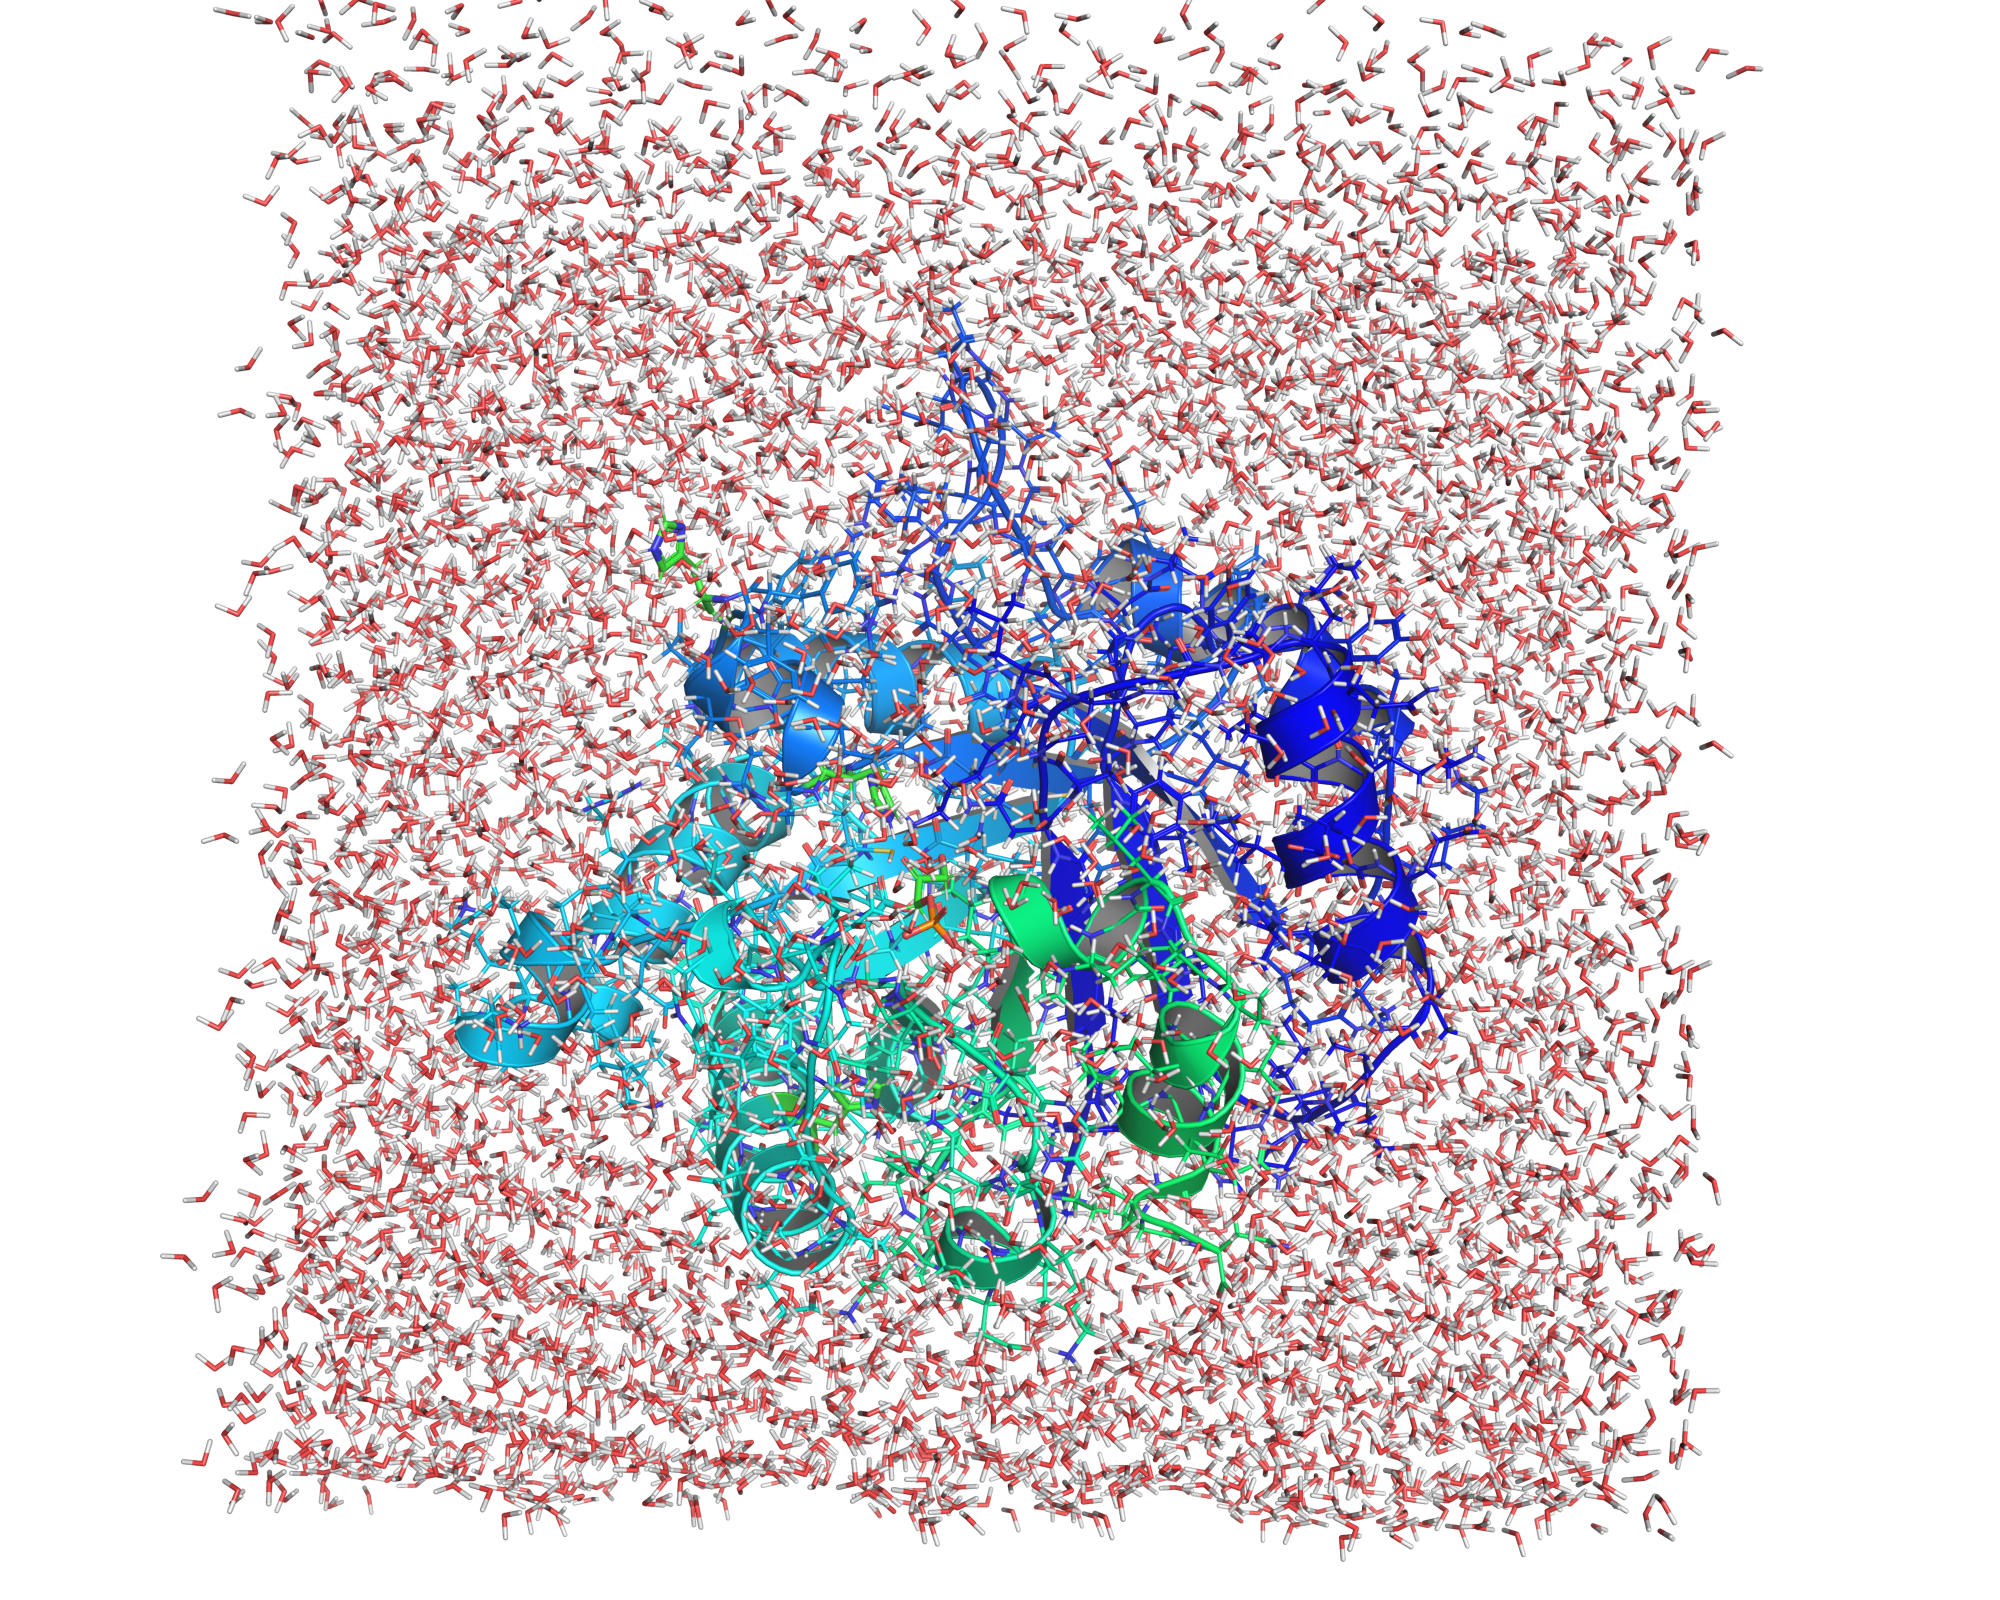
\includegraphics[width=4in]{system_full}
				\caption{Caixa de simulação, contendo a proteína, substrato e moléculas de água.}
				\label{system_full}
			\end{center}
		\end{figure}
	\end{minipage}
	
	\hspace*{-\leftmarginwidth}
	\begin{minipage}{\fullwidth}
		\begin{figure}[H]
			\begin{center}
				\includegraphics[width=4in]{system_prune}
				\caption{Sistema recortado esfericamente a partir do centro reativos, e otimizado com mecânica molecular.}
				\label{system_prune}
			\end{center}
		\end{figure}
	\end{minipage}
	
	\hspace*{-\leftmarginwidth}
	\begin{minipage}{\fullwidth}
		\begin{figure}[H]
			\begin{center}
				\includegraphics[width=4in]{qcmm_opt}
				\caption{Sítio ativo otimizado com QM/MM, pronto para varredura de superfície relaxada.}
				\label{qcmm_opt}
			\end{center}
		\end{figure}
	\end{minipage}
	

 Para esse tutorial será provido um script próprio, que é inspirado em alguns dos testes, com o nome de Reaction\_TIM.py, que pode ser executado com o seguinte comando 
	
	
	\hspace*{-\leftmarginwidth}
	\begin{minipage}{\fullwidth}
		\begin{commandshell}python3 Reaction\_TIM.py\end{commandshell}
	\end{minipage}

	Com esse comando, todos as simulações já enumeradas serão executadas. No entanto, para esse tutorial, vamos fornecer os arquivos com os resultados das simulações até a simulação de varredura de coordenada de reação, que iremos acompanhar durante o mini-curso, devido a duração das simulações de otimizações de geometria. 
	
	Mas antes, vamos analisar cada função dentro do script e entender os parâmetros necessários. (Atividade durante o mini-curso)
	
	
	\subsection{Análise dos Resultados das Simulações}
	
	Esse tutorial ensina a gerar uma trajetória para um caminho de reação e obter os dados de estrutura eletrônica para uma análise posterior no PRIMoRDia. No entanto, podemos verificar algumas métricas e gráficos que foram gerados pelo pDynamo\_scripts, que são os mesmos dados que podem ser utilizados para estudar qualquer caminho de reação. 
	
	Durante essa aula do mini-curso, nós vamos avaliar:
	
	\begin{enumerate}
		\item O gráfico de energia potencial em função do deslocamento da coordenada de reação (\autoref{scantraj})
		\item O gráfico de energia potencial para todos os métodos semi-empíricos no qual o sistema teve a energia refinada considerando uma região tratada por mecânica quântica maior (\autoref{mopac}) .
		\item A renderização da animação da trajetória no Pymol.
	\end{enumerate}
	
	Vemos que o pico de energia potencial se dá antes da transferência do hidrogênio. Essa reação, da forma como foi configurada para ser realizada, é um teste do pDynamo, e ainda não está em condições ótimas, pois a área quântica poderia ser modificada para a varredura, incluindo ou excluindo efeitos importantes. Um dos usos da análise com os descritores é justamente a confirmação dos mecanismos propostos nas análises de superfície de energia potencial.
	
	\hspace*{-\leftmarginwidth}
	\begin{minipage}{\fullwidth}
		\begin{figure}[H]
			\begin{center}
				\includegraphics[width=4in]{ScanTraj}
				\caption{Variação da energia potencial durante a varredura da coordenada de reação, calculadas com potencial híbrido QM/MM com o semi-empírico RM1.}
				\label{scantraj}
			\end{center}
		\end{figure}
	\end{minipage}

	

	\hspace*{-\leftmarginwidth}
	\begin{minipage}{\fullwidth}
		\begin{figure}[H]
			\begin{center}
				\includegraphics[width=4in]{energy}
				\caption{Refinamento de energia}
				\label{mopac}
			\end{center}
		\end{figure}
	\end{minipage}
		
	
	
	\section{Tutorial 3: Análise de Reatividade de Caminho de Reação Enzimático}
	
	Esse tutorial é idêntico ao tutorial 5 do repositório, com a diferença que a trajetória de reação enzimática analisada é que foi gerada no tutorial 2 do presente documento.
		
	Os arquivos necessários para os cálculos desse tutorial estão na pasta. São arquivos de ".aux" e ".pdb", para as etapas do caminho de reação.  Como foram vários métodos semi-empíricos rodados no refinamento de energia no Mopac, foram gerados aquivos com nomes dos Hamiltonianos. Vamos renomear os arquivos de .aux que foram gerados com o RM1 e os respectivos arquivos de PBB para tirar o nome do Hamiltoniano para o PRIMoRDiA reconhecer a sequência de frames, usando os seguintes comandos
	
	\hspace*{-\leftmarginwidth}
	\begin{minipage}{\fullwidth}
		\begin{commandshell}for file in *rm1.aux; 
  do 
    mv "$file" "${file/_rm1.aux/.aux}";
done	\end{commandshell}
	\end{minipage}

	\hspace*{-\leftmarginwidth}
\begin{minipage}{\fullwidth}
	\begin{commandshell}for file in *rm1.pdb; 
  do 
    mv "$file" "${file/_rm1.pdb/.pdb}";
done\end{commandshell}
\end{minipage}
	 
	 
	Para fazer as análises especiais para a reação enzimática teremos que usar outro método de execução, que é sinalizado no PRIMoRDiA pela keyword "reaction" depois de "\#RT" na primeira linha, ou seja, o Run Type passa para o modo de reação. Na pasta já tem o arquivo de input, que agora possui vários elementos importantes de citar, e está mostrado na figura abaixo
	  
	É possível perceber que tem varias outras linhas com keywords antes não usadas e somente uma entrada de arquivo ".aux" para rodar com a opção 3 de cálculo. Como esse é um cálculo para reação química, o PRIMoRDiA entende aquela entrada como valendo para todos os auxs na pasta que tenham o sufixo sinalizado, nesse caso no nosso input foi o sufixo "frame", rodando do "frame0.aux" até o "frame19.aux", obedecendo o parâmetro "dimX".
	 
	Vamos analisar os outros parâmetros do input
	 
	 \hspace*{-\leftmarginwidth}
\begin{minipage}{\fullwidth}
\begin{lstlisting}[caption={Input editado para execução do tutorial 3},label={tut402}]
#RT reaction 
#PR eband 3 Rscript pymols
#Reaction RC1 137 138 73
#Reaction dimX 20
#TRJ residues 3 4 9
3 frame.aux true 30 10 frame.pdb mopac  0 0 0 0 EW
\end{lstlisting}
\end{minipage}
	 
	 Segunda linha
	 \begin{itemize}
	 	\item Segunda linha
	 	\begin{itemize}
	 		\item \#PR:    flag para sinalizar que serão dados parâmetros para o PRIMoRDiA
	 		\item eband:   keyword sinalizando que o próxima parâmetro é um valor de energia de corte para considerar os orbitais moleculares
	 		\item Rscript: keyword importante par gerar os scripts de análise dos descritores durante a trajetória de reação
	 		\item pymols:  keyword para o output de scripts para o Pymol
	 	\end{itemize}
	 	\item Terceira linha
	 	\begin{itemize}
	 		\item \#Reaction: flag para sinalizar que vai ser passado parâmetros para análise de coordenada de reação
	 		\item RC1: keyword sinalizando que vais ser passado o número dos átomos que compõem a coordenada de reação
	 		\item 9:  número do átomo de carbono C1 (C02 no PDB) do GAP 
	 		\item 107:número do átomo de hidrogênio H1 (H02 no PDB) ligado ao DHAP
	 		\item 51: número do átomo de oxigênio OE2 do GLU
	 	\end{itemize}
	 	\item Quarta Linha
	 	\begin{itemize}
	 		\item \#Reaction: flag para sinalizar que vai ser passado parâmetros para análise de coordenada de reação
	 		\item dimX      : keyword para sinalizar que o próximo valor na linha da o número de etapas da trajetória
	 		\item 20        : número de etapas da trajetória
	 	\end{itemize}
	 	\item Quinta Linha 
	 	\begin{itemize}
	 		\item \#TRJ: flag para sinalizar que vai ser passado parâmetros tratar com o conjunto de frames que compõem a trajetória de reação
	 		\item residues    : keyword indicando que os próximos valores inteiros passados nessa linha são o número dos resíduos no PBD que se deseja analisar para a dada trajetória.
	 		\item 3: número no PDB da histidina catalítica
	 		\item 4: número no PDB do Glutamato catalítico
	 		\item 9: número no PDB do resíduo representando o substrato.  
	 	\end{itemize}
	 	\item Sexta Linha 
	 	\begin{itemize}
	 		\item 3      : opção de cálculo do PRIMoRDiA para macromoléculas
	 		\item frame.aux: nome base para os arquivos, antes do ponto o prefixo sem o número que indica o frame, e depois do ponto a extensão do arquivo
	 		\item true   : keyword sinalizando que nenhum métodos de dureza local foi pedido para cálculo da representação volumétrica
	 		\item 30      : finura do grid para representação volumétrica, sempre deixar em zero até uma nova atualização do software
	 		\item 10     : número máximo de orbitais moleculares de fronteira para ser utilizado se o método de combinação de orbitais for BD
	 		\item frame.pdb: nome base para os arquivos de pdb, mesma lógica para os arquivos que contém a estrutura eletrônica
	 		\item mopac  : nome do programa de onde foi calculada a estrutura eletrônica
	 		\item 0      : parâmetro não relevante com grid 0
	 		\item 0      : parâmetro não relevante com grid 0
	 		\item 0      : parâmetro não relevante com grid 0
	 		\item 0      : parâmetro não relevante com grid 0
	 		\item EW     : keyword para o método de combinação de orbitais moleculares
	 	\end{itemize}
	 \end{itemize}
	 
	 \subsection{Análise dos Resultados}
	 
	 Para analisar todos os descritores e outras propriedades de energia, o PRIMoRDiA cria um script para executar no R que por sua vez produz gráficos dessas quantidades variando em função das frames. Depois da execução deve aparecer arquivos com sufixo ".R", um deles com nome "frame0\_reaction\_analysis.R" e outro "frame0\_residuos\_analysis.R". Vamos executar o primeiro com o Rscript, como no comando abaixo
	 
	 \hspace*{-\leftmarginwidth}
	 \begin{minipage}{\fullwidth}
	 	\begin{commandshell}Rscript frame0\_reaction\_analysis.R\end{commandshell}
	 \end{minipage}
	 
	 Depois desse comando, o R deve produzir diversos arquivos de imagem com propriedades globais e locais para cada átomo da coordenada de reação. No primeiro gráfico da \autoref{fig_tut5_2} HOF é o calor de formação (heat of formation) que o Mopac calcula, e é uma das melhores formas de variação de energia em uma reação química simulada com método semi-empírico. Lembrado que todas essas propriedades são em referência ao primeiro valor, ou seja, cada ponto uma variação ao estado inicial. Nessas simulações uma estrutura que normalmente se deseja determinar é a estrutura de transição, que é determinada pelo ponto máximo de variação de energia, nesse caso na penúltima etapa. No entanto, nesse nosso calculo com PM6, a área quântica foi bem menor do que a utilizada no na nossa publicação e o HOF não foi um bom indicador do estado de transição. Já a energia eletrônica mostra um primeiro máximo no ponto zero da coordenada de reação, que é o momento que o próton está a mesma distância do carbono e do oxigênio. Em geral, os outros descritores globais indicam um aumento da moleza química (softness) e consequente diminuição da dureza (hardness), aumento do potencial químico e da eletrofilicidade total indicam que o sistema tende a receber transferência de elétrons.
	 
	 \hspace*{-\leftmarginwidth}
	 \begin{minipage}{\fullwidth}
	 	\begin{figure}[H]
	 		\begin{center}
	 			\includegraphics[width=4in]{global_rc1}
	 			\caption{Descritores globais calculados para cada etapa da trajetória de reação.}
	 			\label{fig_tut5_2}
	 		\end{center}
	 	\end{figure}
	 \end{minipage}
	 	 
	 	 
	 Na \autoref{fig_tut5_4}, nós mostramos os descritores para o átomo de oxigênio do resíduo GLU. No script gerado pelo PRIMoRDiA nós analisamos 9 propriedade por átomo da coordenada de reação. Para o oxigênio é interessante ressaltar algumas, como o decréscimo na densidade eletrônica, atingindo um mínimo no estado de transição e depois retomando o valor nos produtos. A carga parcial aumenta também, indicando que há uma transferência de elétrons do oxigênio para o carbono, e que depois o sistema em volta faz uma "devolução" de carga para o oxigênio, mas que no final ainda fica com menos, já que agora o grupo carboxílico está protonado e portanto neutro. Já para a dureza local esse átomo apresenta comportamentos diferentes para cada tipo de método de cálculo, para interpretar o que cada um significa é importante entender cada modelo. Brevemente, a dureza baseada no LCP tem mais correção com o descritor global de dureza, indicando que esse tinha a propensão de interagir por processo duro-duro e depois foi diminuindo esse comportamento conforme foi transferindo carga. 
	 
	 \hspace*{-\leftmarginwidth}
	 \begin{minipage}{\fullwidth}
	 	\begin{figure}[H]
	 		\begin{center}
	 			\includegraphics[width=4in]{la_0}
	 			\caption{Descritores locais calculados para o átomo O2E do grupo carboxílico do Glutamato catalítico para a trajetória de reação.}
	 			\label{fig_tut5_4}
	 		\end{center}
	 	\end{figure}
	 \end{minipage}
	 
	 
	 Os descritores para o carbono C1 estão na \autoref{fig_tut5_5}. Tem bastante coisa interessante para analisar nesse caso. Primeiro, como que para dois métodos de dureza o valor máximo condiz com o estado de transição e se assemelha bastante com o perfil de energia da reação. Já que a interação dominante para transferência de prótons é a duro-duro, o carbono assume o valor máximo para esse descritor, em dois métodos Vee e LCP. O método de dureza baseado no potencial de Fukui da a força exercida nos núcleos em respeito da varição do número de elétrons, o que tem una interpretação mais diferente da geral sobre dureza comum. 
	 
	 \hspace*{-\leftmarginwidth}
	 \begin{minipage}{\fullwidth}
	 	\begin{figure}[H]
	 		\begin{center}
	 			\includegraphics[width=4in]{la_1}
	 			\caption{Descritores locais calculados para o átomo C1 do substrato para a trajetória de reação.}
	 			\label{fig_tut5_5}
	 		\end{center}
	 	\end{figure}
	 \end{minipage}
	 
	 Os descritores para o átomo transferido, o hidrogênio do DHAP (H1), se encontra na figura de baixo. Os descritores baseados nos orbitais moleculares, como eletrofilicidade, nucleofilicidade e netfilicidade mostraram variação mas com valores muito baixos. Agora é interessante como a densidade eletrônica vai diminuindo, se tornando cada vez mais um próton, um hidrogênio carregado positivamente. A dureza local calculado pela aproximação do potencial de Fukui, foi a que apresentou maior coerência com o processo, com um aumento das interações eletrostáticas próximo ao estado de transição, diminui e atinge o máximo nos produtos, onde a carga parcial alcança o maior valor, sendo que esse átomo tende a ser transferido pelo mesmo tipo de interação.
	 
	 \hspace*{-\leftmarginwidth}
	 \begin{minipage}{\fullwidth}
	 	\begin{figure}[H]
	 		\begin{center}
	 			\includegraphics[width=4in]{la_2}
	 			\caption{Descritores locais calculados para o átomo H1 do substrato para a trajetória de reação.}
	 			\label{fig_tut5_6}
	 		\end{center}
	 	\end{figure}
	 \end{minipage}
	 
	 
	 Como no Tutorial 3, vamos gerar imagens do descritores para alguns pontos da trajetória. O PRiMoRDiA escreve para cada arquivo um script de Pymol para automatizar a visualização dos descritores. Abra o Pymol e execute o arquivo com o prefixo "frame0" e sufixo ".pym". Como mostrado na \autoref{fig_tut5_6} e no caixa de comando abaixo. 
	 
	 \hspace*{-\leftmarginwidth}
	 \begin{minipage}{\fullwidth}\begin{pymol}@frame0_pymols.pym\end{pymol}
	 \end{minipage}
	 
	 \hspace*{-\leftmarginwidth}
	 \begin{minipage}{\fullwidth}
	 	\begin{figure}[H]
	 		\begin{center}
	 			\includegraphics[width=4in]{frame0_descritores}
	 			\caption{Janela do Pymol com os resultados dos descritores carregados e o objeto do descritor de .}
	 			\label{fig_tut6_6}
	 		\end{center}
	 	\end{figure}
	 \end{minipage}
 
     \hspace*{-\leftmarginwidth}
     \begin{minipage}{\fullwidth}
     	\begin{figure}[H]
     		\begin{center}
     			\includegraphics[width=4in]{frame0_homo}
     			\caption{Janela do Pymol com a representação volumétrica do orbital HOMO.}
     			\label{fig_homo}
     		\end{center}
     	\end{figure}
     \end{minipage}
	 
	 Esses descritores em representação volumétrica são esteticamente apelativos, mas apresentam um custo computacional alto e podem apresentar uma visualização mais confusa quando o restante da estrutura da proteína é apresentada. Para gerar representações de descritores centrada nos átomos pode ser utilizado o outro script gerado também pelo PRIMoRDiA, com o seguinte comando no software pymol
	 
	  \hspace*{-\leftmarginwidth}
	 \begin{minipage}{\fullwidth}\begin{pymol}@frame0_pymols_pdb.pym\end{pymol}
	 \end{minipage}
	 
	 	 
	 As próximas figuras foram resultado do processo de renderização no pymol para o descritor de dureza local com o segundo método disponível no PRIMoRDiA. O objeto com a proteína inteira foi colorido com os carbonos em verde e escondido todas as outras representação que não fossem cartoon para não atrapalhar a visualização do objeto com o descritor. Para a palheta escolhida o comando utilizado foi 
	 
	 \hspace*{-\leftmarginwidth}
	 \begin{minipage}{\fullwidth}\begin{pymol}spectrum b, white_yellow_orange_red_black, minimum=0.1,maximum=0.2
	 	\end{pymol}
	 \end{minipage}
	 
	 
	 Esses valores podem sofrer pequenos ajustar para melhorar o destaque dos átomo com o maior valor de dureza. Depois, com o comando "ray" seguido do "png" as imagens foram salvas. A \autoref{fig_tut6_8} mostra a dureza local para a primeira etapa da coordenada. Durante o tutorial, abriremos outras estruturas e faremos as renderizações dos outros descritores. 
	 
	 
	 \hspace*{-\leftmarginwidth}
	 \begin{minipage}{\fullwidth}
	 	\begin{figure}[H]
	 		\begin{center}
	 			\includegraphics[width=4in]{frame0_hardness}
	 			\caption{Dureza local para os átomos da enzima tratados com mecânica quântica para a estrutura corresponde ao primeiro passo da trajetória de reação. }
	 			\label{fig_tut6_8}
	 		\end{center}
	 	\end{figure}
	 \end{minipage}
	 
	 
	 O PRIMoRDiA também escreve scripts especiais do R para a análise dos descritores para residuos específicos, indicados no input, produzindo gráficos de barra com a média e o desvio padrão, como na figura abaixo para o descritor de eletrofilicidade local  na \autoref{fig_tut6_11}, nucleofilicidade local na \autoref{fig_tut6_12}.
	
	 
	 \hspace*{-\leftmarginwidth}
	 \begin{minipage}{\fullwidth}
	 	\begin{figure}[H]
	 		\begin{center}
	 			\includegraphics[width=3in]{Eph_res}
	 			\caption{Gráfico de barras para a eletrofilicidade nos residuos indicados durante a trajetória.}
	 			\label{fig_tut6_11}
	 		\end{center}
	 	\end{figure}
	 \end{minipage}
	 
	 
	 \hspace*{-\leftmarginwidth}
	 \begin{minipage}{\fullwidth}
	 	\begin{figure}[H]
	 		\begin{center}
	 			\includegraphics[width=3in]{Nph_res}
	 			\caption{Gráfico de barras para a Nucleofilicidade nos residuos indicados durante a trajetória.}
	 			\label{fig_tut6_12}
	 		\end{center}
	 	\end{figure}
	 \end{minipage}
	 
	 
	 Também, é acompanhado a variação desses valores durante a trajetória com o cálculo de médias móveis, como na \autoref{fig_tut6_13} é mostrado para densidade eletrônica em cada resíduo indicado no input, para a dureza local na \autoref{fig_tut6_14} e moleza local\autoref{fig_tut6_15}. 
	 
	 \hspace*{-\leftmarginwidth}
	 \begin{minipage}{\fullwidth}
	 	\begin{figure}[H]
	 		\begin{center}
	 			\includegraphics[width=4in]{net_mov_avg}
	 			\caption{Médias móveis para a densidade eletrônica para os residuos indicados no input para análise da trajetória.}
	 			\label{fig_tut6_13}
	 		\end{center}
	 	\end{figure}
	 \end{minipage}
	 
	 \hspace*{-\leftmarginwidth}
	 \begin{minipage}{\fullwidth}
	 	\begin{figure}[H]
	 		\begin{center}
	 			\includegraphics[width=4in]{Hsoftness_mov_avg}
	 			\caption{Médias móveis para o descritor de Hiper moleza local para os residuos indicados no input para análise da trajetória.}
	 			\label{fig_tut6_14}
	 		\end{center}
	 	\end{figure}
	 \end{minipage}
	 
 
	 
	 Há diversas análises que podemos fazer baseados nos descritores de reatividade, que por sua vez também são numerosos, para cada átomo envolvido e para cada resíduo. O PRIMoRDiA fornece uma forma automática de dispor todos esses resultados da forma mais pronta para análise possível. 
	
	\section{Considerações Finais}
	
	\newpage
	\section*{Agradecimentos}
	
	We gratefully thanks the Brazilian science/education institutes by the physical structure and financial support: INCT-INAMI, CNPq,CAPES,FAPESQ-PB, PRONEX-FACEPE and FINEP. Universidade Federal da Paraíba (UFPB) and the computer resources of Centro Nacional de Processamento de Alto Desempenho em São Paulo (CENAPAD-SP). 		
	Research project Bioinformática Estrutural de Proteínas: Modelos, Algoritmos e Aplicações Biotecnológicas (Edital Biologia Computacional 51/2013, processo AUXPE1375/2014 da CAPES). G.B.R. acknowledges support from the Brazilian National Council for Scientific and Technological Development (CNPq grant no. 309761/2017-4).
	
	
	
	\bibliographystyle{ieeetr}
	\newpage
	\bibliography{refs}
	
	
\end{document}
